\documentclass[10pt,titlepage,a5paper]{ltjsbook}
\usepackage{amsmath}
\usepackage{amssymb}
\usepackage{amsfonts}
\usepackage{graphicx}
\usepackage{float}
\usepackage{xcolor}
\usepackage{enumitem}
\usepackage{etoolbox}
\usepackage{subfiles}
\usepackage{cleveref}
\usepackage{tcolorbox}
\usepackage{quotchap}
\usepackage{fancyhdr}
\usepackage{wrapfig}
\usepackage{geometry} % geometry パッケージを読み込む
\geometry{
    a5paper,      % 用紙サイズを再度指定(冗長でも安全のため)
    left=12mm,    % 左の余白を12mmに
    right=12mm,   % 右の余白を12mmに
    top=12mm,     % 上の余白を12mmに
    bottom=12mm,  % 下の余白を12mmに
    %showframe % 余白の境界線を可視化したい場合(最終出力時には削除)
}
\usepackage{titlesec}
\titleformat{\section}[block]{}{}{0pt}
{
  \definecolor{teal}{gray}{0.30}
  \begin{picture}(0,0)
    \put(-10,-5){
      \begin{tikzpicture}
        \fill[teal] (0pt,0pt) rectangle (5pt,19pt);
      \end{tikzpicture}
    }
    \put(-10,-5){
      \color{teal}
      \line(1,0){\hsize}
    }
  \end{picture}
  \hspace{0pt}
  \sffamily \Large \thesection
  \hspace{0pt}
}
\pagestyle{fancy} % fancy スタイルを使用することを宣言

% ヘッダーとフッターのすべてのフィールドをクリア
\fancyhf{}

% 奇数ページ (odd page) のフッター設定
\fancyfoot[LO]{\thepage} % Left Odd: 左下 (ページ番号)
\fancyfoot[RO]{}         % Right Odd: 右下 (空にする)

% 偶数ページ (even page) のフッター設定
\fancyfoot[LE]{}         % Left Even: 左下 (空にする)
\fancyfoot[RE]{\thepage} % Right Even: 右下 (ページ番号)

% ヘッダーとフッターの下線を消す
\renewcommand{\headrulewidth}{0pt} % ヘッダーの下線を0pt (消去)
\renewcommand{\footrulewidth}{0pt} % フッターの上線を0pt (消去)

% chapter の開始ページ(plain スタイル)もフッターにページ番号を表示させる
\fancypagestyle{plain}{
  \fancyhf{} % ヘッダーとフッターをクリア
  \fancyfoot[LO]{\thepage} % 左下 (奇数ページ)
  \fancyfoot[RE]{\thepage} % 右下 (偶数ページ)
  \renewcommand{\headrulewidth}{0pt} % ここにも下線消去を設定
  \renewcommand{\footrulewidth}{0pt} % ここにも下線消去を設定
}
\begin{document}
\chapter{屋久島の生物}
\section{垂直分布}
  前章で解説したように, 屋久島はその狭い島に海辺の亜熱帯から山頂の亜寒帯までの気候を持つ. この気候に起因して, 屋久島は標高によって植生が異なる. これを\textbf{垂直分布}\footnotemark[6] \footnotetext[6]{屋久島が世界自然遺産に登録された要因の一つとされる.}と呼ぶ.
  植生の分布としては0-200mは亜熱帯林·海岸林, 200-600mは照葉樹林, 600-1000mの下層では常緑の広葉樹が繁茂し, 上がっていくと次第に針葉樹が増えていく. 1000-1700mではほぼ屋久杉だけになり, 1700mを超えると森林限界でヤクザサなどの背の低い草本が生育する. 
\section{屋久島の森の主役:屋久杉}
  屋久島の植物の代表は紛れもなく屋久杉であろう. 屋久杉とは屋久島に生え, 樹齢1000年以上の杉の総称である. 1000年未満のものは小杉と呼ばれ, 人工的に植林されたものは地杉と呼ぶ.屋久杉が長寿な理由として, 1. 強風, 2.花崗岩質の土壌, 3.多雨などに由来して生長が非常に遅く緻密で, 樹脂が多く含まれるからである. \\
  \subsection{有名な屋久杉}
  屋久島には有名な屋久杉がいくつもある. その中でも特に有名なものを紹介する.
  \begin{minipage}{0.38\columnwidth}
    \begin{figure}[H]
      \centering
      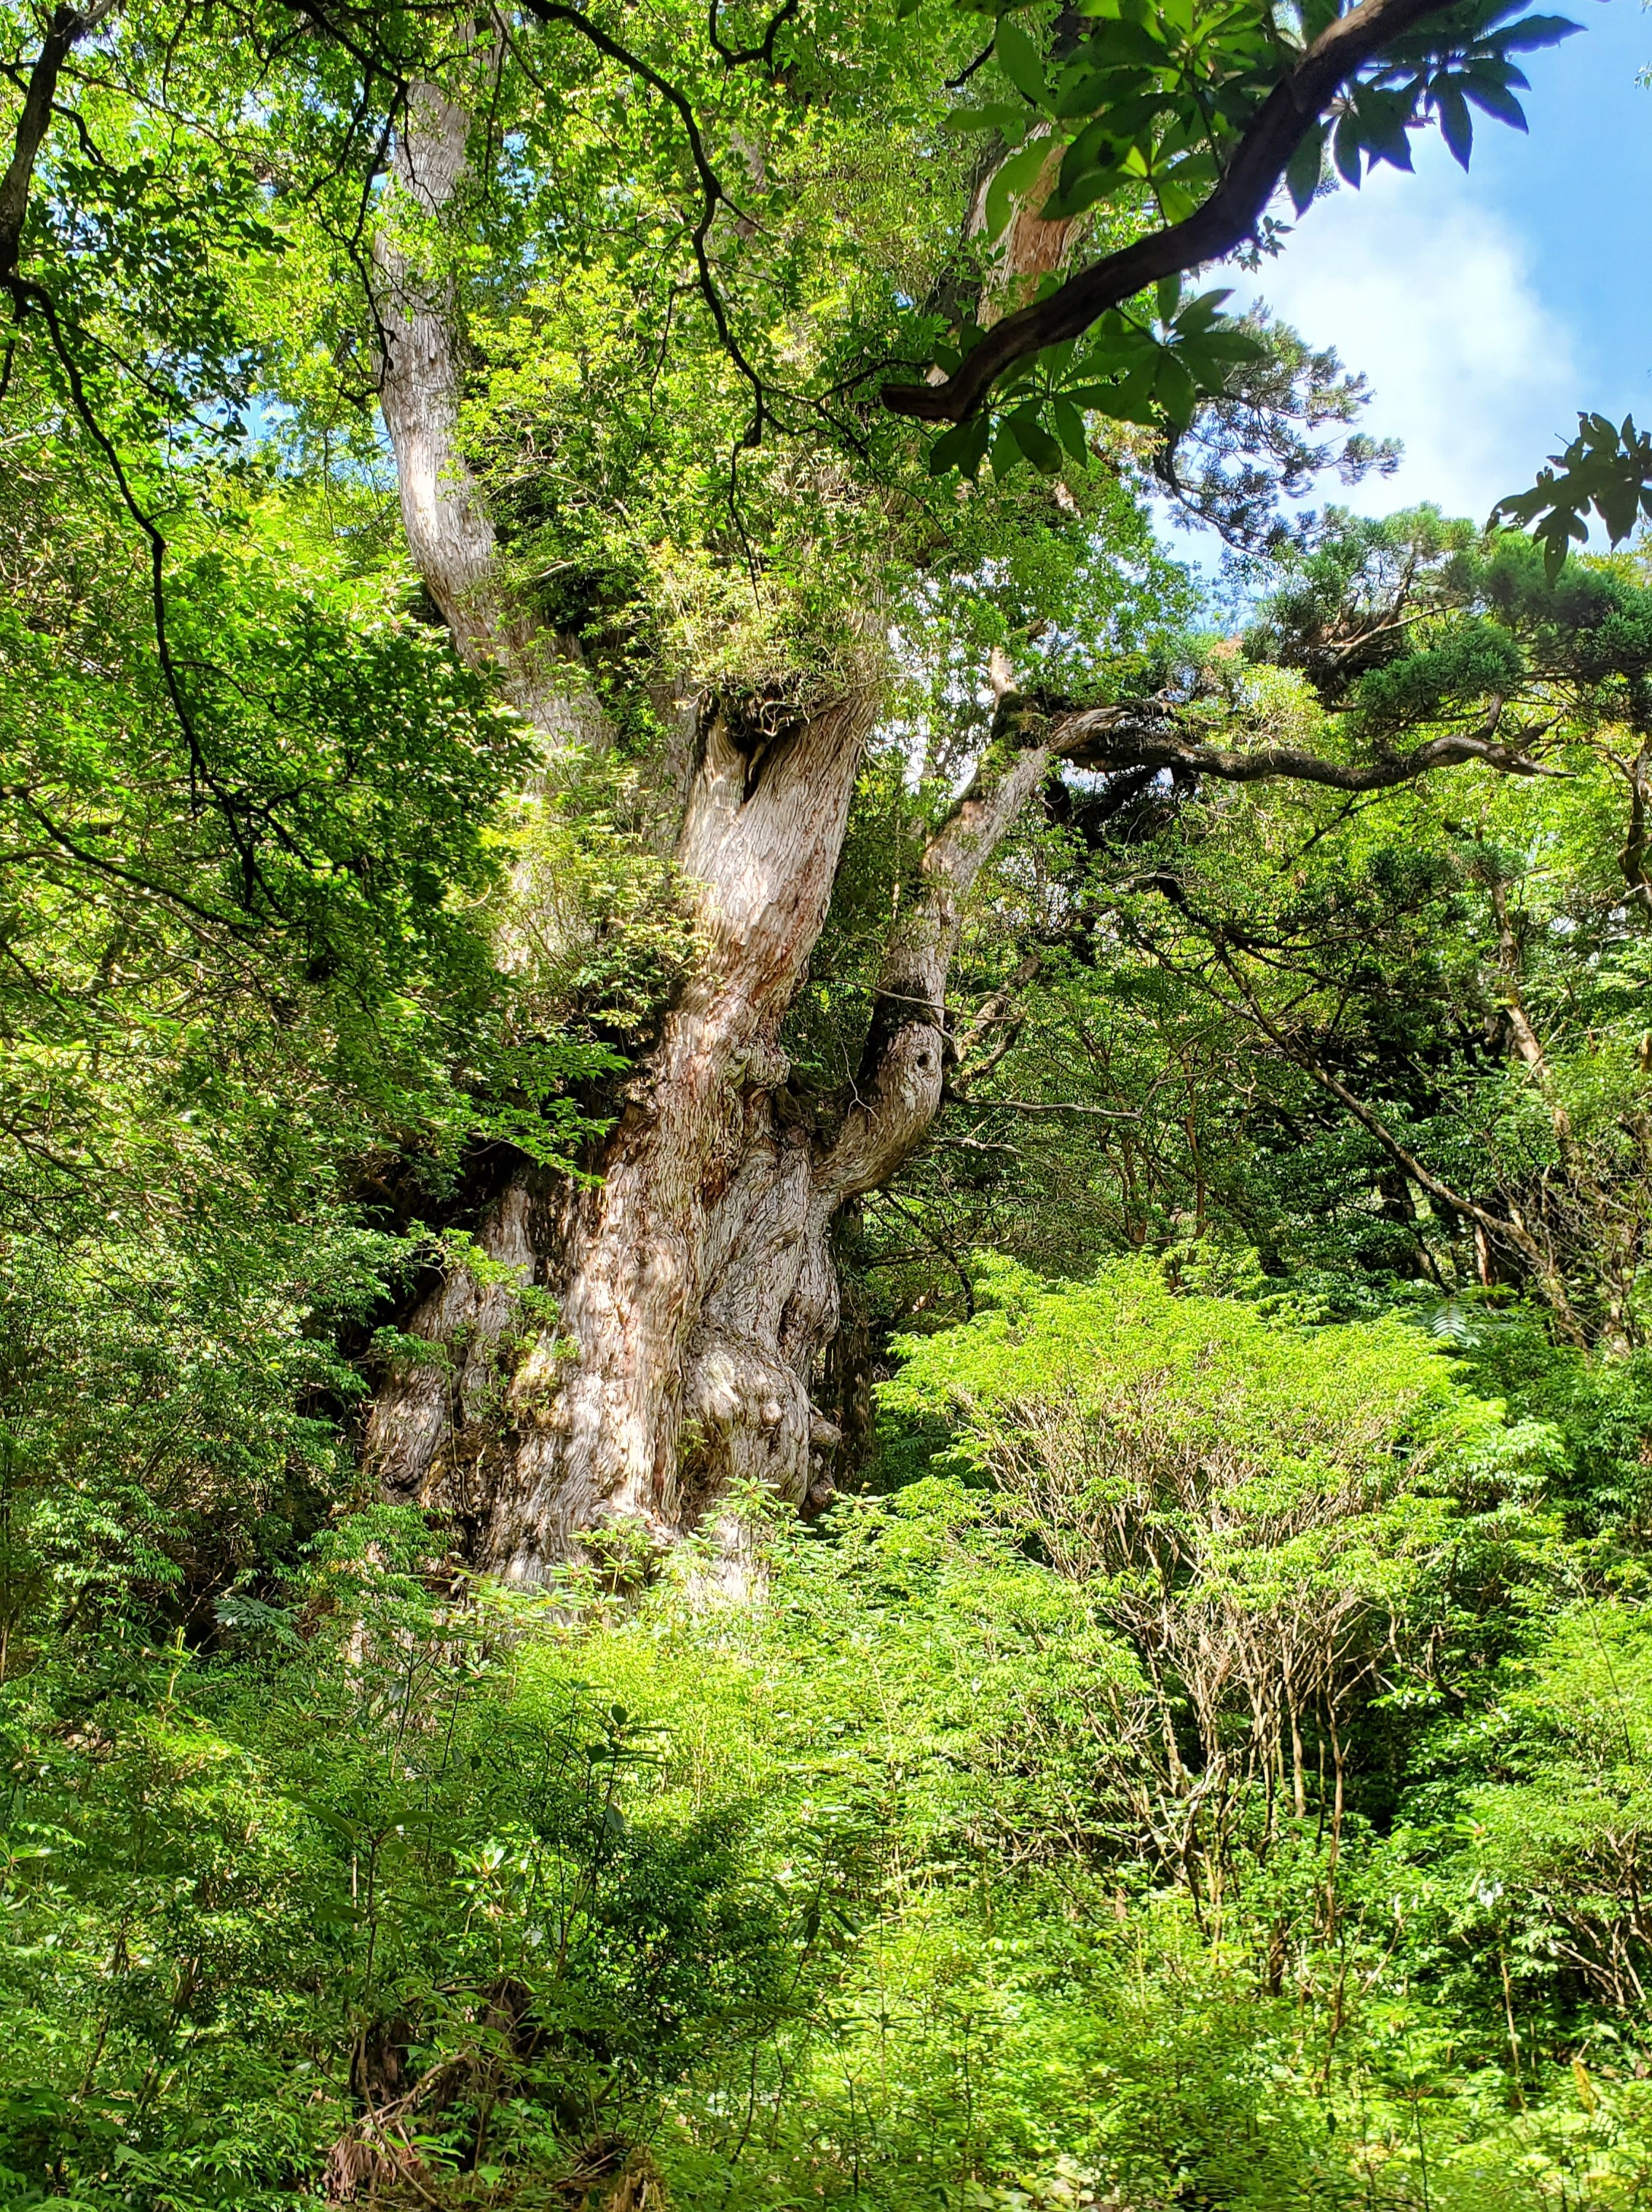
\includegraphics[width=\columnwidth]{joumon.jpg}
      \caption{縄文杉の写真}
      \label{fig:jomon_photo}
    \end{figure}
  \end{minipage}
  \hfill
  \begin{minipage}{0.58\columnwidth}
    \subsubsection*{縄文杉}
      縄文杉は, 屋久島の象徴ともいえる存在であり, 樹齢は2000年から7200年と幅広い\footnotemark[7]. 樹高は30m, 幹周りは16.4mである. 発見当初は触るほどの距離に行くことができたが, 
      根の保護のために展望デッキからしか見れないようになっている. ここへのトレッキングコースは屋久島のトレッキングコースの中でも最も人気があり, 多い年で年間9万人以上が訪れていたが現在は5万人程度に減少している.一度は見てほしいとは思うが, 見てみると遠くてよくわからない.
  \end{minipage}
  \footnotetext[7]{詳しくはコラムを参照のこと.}
  \begin{minipage}{0.58\columnwidth}
    \subsubsection*{大王杉}
      大王杉は, 樹齢3000年, 樹高23m, 幹周りは11.6mである. 縄文杉発見以前は屋久島で最も大きい屋久杉であった. 縄文杉に向かう道の途中にあり, 縄文杉より近くで見ることができる. その迫力はまさに大王という名にふさわしく,個人的には縄文杉よりも迫力を感じた.
  \end{minipage}
  \hfill
  \begin{minipage}{0.38\columnwidth}
    \begin{figure}[H]
          \centering
          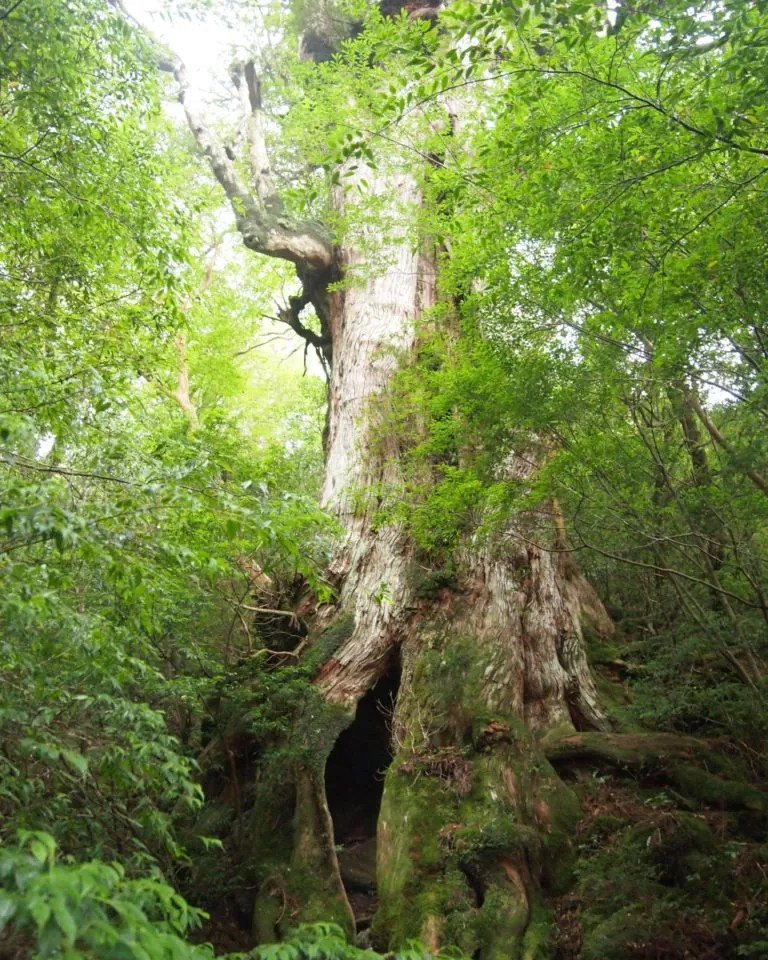
\includegraphics[width=\columnwidth]{daioh.jpg}
          \caption{大王杉の写真}
          \label{fig:daioh_photo}
      \end{figure}
  \end{minipage}
  \begin{minipage}{0.38\columnwidth}
    \begin{figure}[H]
          \centering
          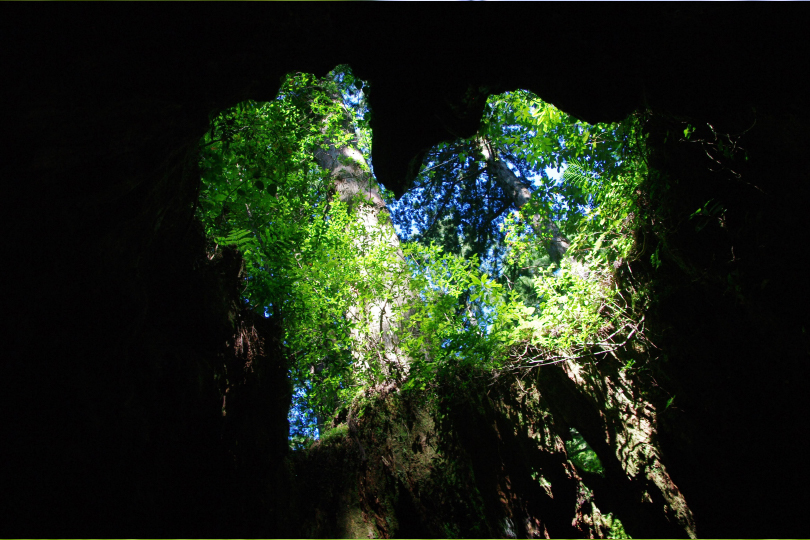
\includegraphics[width=\columnwidth]{willson.jpg}
          \caption{ウィルソン株の写真}
          \label{fig:willson_photo}
      \end{figure}
  \end{minipage}
  \hfill
  \begin{minipage}{0.58\columnwidth}
    \subsubsection*{ウィルソン株}
      ウィルソン株は, 伐採時の推定樹齢3000年, 高さ5m, 幹周りは13.8mの屋久島最大の切株である. 1914年に植物学者A.H.Wilsonが発見したことから名がつけられた. 内部からハートのように写真を撮ることができる. こちらも縄文杉に向かう途中にある.
  \end{minipage}
  \subsection{倒木更新}
    倒木更新とは, 木が倒れた後に, その倒木の上に新たな木が生えてくる現象である. 屋久島では, 土壌の貧栄養ゆえ, 倒木の上に新たな木が生えることが多い. そうすることで, 倒木の栄養を利用し, 下草の影響を受けないため十分に日光を浴びて生長することができる. また, 同じく切り株の上に生える切り株更新というものもある.
  \subsection{着生}
    屋久杉のまわりには, 保水力が高い苔が生えており, その苔の上に植物が生えることが多い. これを着生と呼ぶ. 着生は根が巨木に絡みついているだけで, 寄生ではない. 屋久杉には多くの植物が着生し, 一つの生態系を形成しているのである.
  \vspace{1em}
  \begin{tcolorbox}[title=コラム:縄文杉は何歳?,width=\textwidth]
    縄文杉の樹齢は2000年から7200年と幅がある. 発見当初, その大きさから樹齢7200年と推定されたが, その後の炭素年代測定法では2170年となった. これは内部が空洞になっていて古いサンプルが取れなかったためである.
    また, 古木の周囲を若木2,3本が取り囲むように生えている合体木ではないかともされたが, 調査により, 1本の木であること, 倒木更新の痕跡があることが明らかになった. 前述の幸谷火砕流で, 屋久島のほぼ全域は7200年前に火砕流に覆われたと考えられる. その後1000年は樹木が生えなかったと考えられるため, 縄文杉の前に生えていた木があることを考えると, 樹齢は4000年, 多くても5000年ほどだとされている.
  \end{tcolorbox}
\section{森の植物}
  屋久島には, 多くの植物が生育している. その中でも特に有名なものを紹介する.
  \subsection{沿岸の植物}
    \begin{minipage}{0.38\columnwidth}
      \begin{figure}[H]
            \centering
            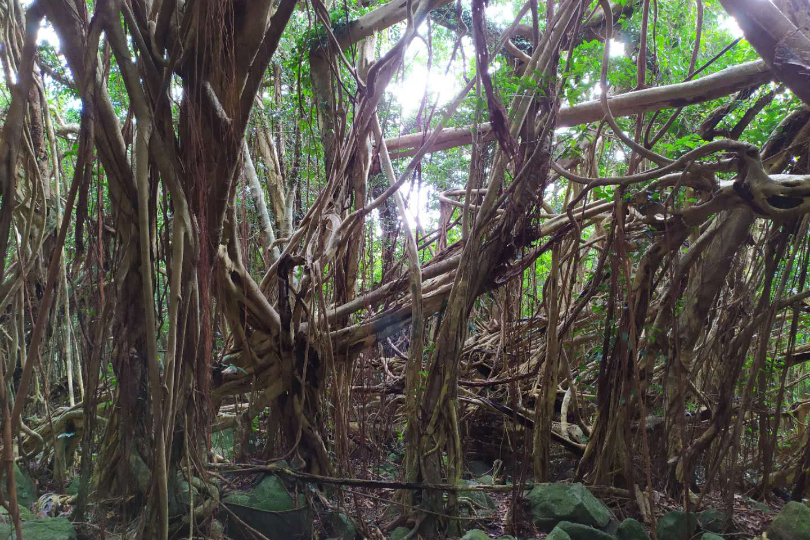
\includegraphics[width=\columnwidth]{gajumaru.jpg}
            \caption{ガジュマルの写真}
            \label{fig:gajumaru_photo}
        \end{figure}
    \end{minipage}
    \hfill
    \begin{minipage}{0.58\columnwidth}
      \subsubsection*{ガジュマル}
      ガジュマルは, 亜熱帯から熱帯に分布する常緑高木である. 特徴として, 枝から根(気根)が垂れ下がり, 地面に達すると根を張る. これにより, 特徴的な見た目を形成する. 登りやすい. 屋久島では, 沿岸のいたるところで見られる.
    \end{minipage}
    \begin{minipage}{0.58\columnwidth}
      \subsubsection*{アコウ}
        ガジュマルに似た植物で, 中学校に大きな木があった. アコウも気根を持つが, ガジュマルほど太くならない. しばしばほかの植物に着生し, 気根で元の木を覆い, 枯らしてしまう. そのため, 絞め殺しの木\footnotemark[8]と呼ばれる.
    \end{minipage}
    \footnotetext[8]{屋久島では, ヤマグルマも同様に絞め殺しの木と呼ばれる.}
    \hfill
    \begin{minipage}{0.38\columnwidth}
      \begin{figure}[H]
            \centering
            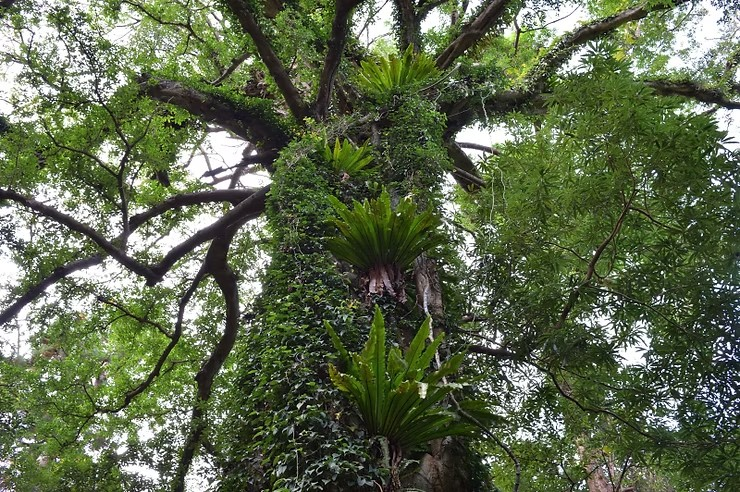
\includegraphics[width=\columnwidth]{akou.jpg}
            \caption{アコウの写真}
            \label{fig:akou_photo}
        \end{figure}
    \end{minipage}
\section{森の動物}
\section{海の生物}
\end{document}